\section{Embedded RT Systems}
\subsection{Charakterisierung Embedded Systems}
Ein Embedded System \ldots
\begin{itemize}
  \item \ldots ist ein System, das einen Computer beinhaltet, aber keiner ist
  \item \ldots besteht üblicherweise aus HW und SW
  \item \ldots ist häufig ein Control System
\end{itemize}
\subsubsection{Charakterisierung von Embedded Systems}
  \begin{itemize}
    \item \textbf{Reaktive Systeme} : Interagieren mit ihrer Umgebung
    \item \textbf{Echtzeitsysteme/Real-time systems} : Definierbare zeitliche
    Anforderungen erfüllen
    \item \textbf{Verlässliche Systeme/Dependable systems}: Sehr hohe
    Zuverlässigkeitsanforderungen erfüllen
    \item \textbf{Weitere Anforderungen/Charakteristiken}: 
    \begin{itemize}
      \item Kleiner Energieverbrauch
      \item Kleine physikalische Abmessungen
      \item Lärm, Vibration, Feuchtigkeit etc.
    \end{itemize}
  \end{itemize}

\subsubsection{Verfügbarkeit}
Anteil der Betriebsdauer, in  der das System seine Funktion
erfüllt: 

\begin{equation}
Verfuegbarkeit = \frac{Gesamtzeit-Ausfallzeit}{Gesamtzeit}
\end{equation}

\subsection{Real-time Systems}
\textbf{Definition} : System, das Informationen innerhalb einer definierten Zeit
(deadline) bearbeiten muss. Es erfüllt explizite Anforderungen an die
Antwortzeiten.\\
\textbf{Antwortzeit} : Zeit vom Stimulus (Vorhandensein
Eingangswert) bis zum Erscheinen des Ausgangswert\\
\textbf{Fehlerhaftes System:} es werden nicht alle formal definierten Systemspezifikationen erfüllt.\\
\textbf{Soft real-time system}: System wird durch das verletzen von
Antwortzeiten nicht ernsthaft beeinflusst $\rightarrow$ Komforteinbussen (Bsp.:
Geldautomat)\\
\textbf{Firm real-time system}: Durch Verletzen weniger Antwortzeiten wird das
System nicht ernsthaft beeinflusst. Bei vielen Verletzungen jedoch $\rightarrow$
kompletter Ausfall, katastrophales Fehlverhalten (Bsp.: GPS-gesteuerter
Rasenmäher)\\
\textbf{Hard real-time system}: Durch Verletzen der Antwortzeiten wird das
System ernsthaft beeinflusst $\rightarrow$ kompletter Ausfall, katastrophales
Fehlverhalten (Bsp.: Helikoptersteuerung)\\
\textbf{Determinismus}: Für jeden möglichen Zustand und alle möglichen
Eingabewerte ist jederzeit der nächste Zustand und die Ausgabewerte definiert.

\begin{multicols}{2}
\textbf{Auslastung/Utilization}: 
Auslastung pro Prozess:
\begin{center}  
\begin{tabular}{c c}
& $u_\text{i}$ = Ausführungsfaktor des Task i\\
$u_\text{i} = \frac{e_\text{i}}{p_\text{i}}$&$e_\text{i}$ = Executionzeit des
Task i\\
& $p_\text{i}$ = Executionperiode des Task i
\end{tabular}\\
\end{center}

\columnbreak

Für n periodische Tasks erhalten wir die gesamte Auslastung U: 
\begin{center}
\begin{equation}
U = \sum_{i=1}^{n}u_\text{i} = \sum_{i=1}^{n}\frac{e_\text{i}}{p_\text{i}}
\end{equation}
\end{center}
\end{multicols}

\subsection{Rate monotonic scheduling (RMS)}
\subsubsection{Cooperative Scheduling}
  \begin{itemize}
    \item Aktiver Task entscheidet selbst, wann er den Prozessor für anderen
    Task frei gibt. 
    \item Ein unfairer Task blockiert dabei die anderen
    \item Nächster Task aussuchen via: FCFS, Round Robin, zufällig, Prioritäten, etc.
    \item Einfach zu implementieren
  \end{itemize}
\subsubsection{Preemptive Scheduling}
  \begin{itemize}
    \item Task mit höherer Priorität wird ausgeführt
    \item Task mit niederer Priorität wird verdrängt (preempt)
    \item Prioritätsverteilungsmöglichkeiten
      \begin{itemize}
        \item Dynamic-priority algorithm: Prioritäten werden zur Laufzeit
        aufgrund vorhandener Deadlines angepasst. 
        \item Static-priority algorithm: Prioritäten werden zur Entwicklungszeit
        festgelegt und nicht mehr geändert. $\rightarrow$ Einfacher als dynamic-priority
      \end{itemize}
    \item Viele RTOS verwenden preemptive static-priority Algorithmen 
  \end{itemize}
\subsubsection{Schedulability}
 Eine Menge von Tasks ist dann schedulable, wenn alle Tasks zu allen Zeiten ihre Deadlines einhalten können.
\subsubsection{Rate-monotonic scheduling}
\textbf{Theorem:} 
Hat man ein Set periodischer Task und preemptive static-priority scheduling,
erhält man optimales Scheduling, wenn man die Prioritäten so verteilt, dass die
Tasks mit kürzester Periodizität die höhere Prioriät erhalten (rate
monotonic).\\
\textbf{Oder:}
Ein Set von n periodischen Tasks ist dann rate-monotonic schedulable, wenn die gesamte Systemauslastung U folgenden Wert nicht überschreitet: 
\begin{equation}
U \leq n\cdot(2^\frac{1}{n}-1)
\end{equation}\\

\begin{tabular}{| l | l | l | l | l | l | l |}
	\hline
	n & 2 & 3 & 4 & 5 & 10 & $\infty$\\
	\hline
	u [\%] & 82.4 & 78.0 & 75.7 & 74.4 & 71.7 & 69.3 \\
	\hline
\end{tabular}\\\\
	
Die maximale Systemauslastung beträgt: 
\begin{equation}
\lim_{n \to \infty}n\cdot(2^\frac{1}{n}-1) = \ln 2 \approx 0.69
\end{equation}
Folgerung aus diesem Grenzwert: Das theoretische Limit der Systemauslastung
liegt bei 69\%. 
\subsubsection{Beispiel RMS}
\begin{minipage}[t]{4 cm}
	\begin{tabular}{| l | l | l | l |}
		\hline
		$\tau_i$ & $e_i$ & $p_i$ & $u_i=\frac{e_i}{p_i}$ \\
		\hline
		$\tau_1$ & 1 & 4 & 0.25 \\
		\hline
		$\tau_2$ & 2 & 5 & 0.4 \\
		\hline
		$\tau_3$ & 5 & 20 & 0.25 \\
		\hline
	\end{tabular}
\end{minipage} 
\begin{minipage}[c]{14 cm}		
	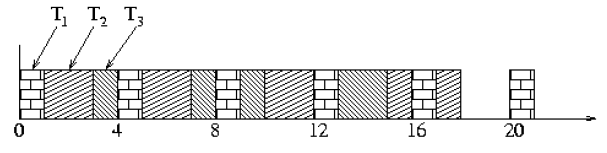
\includegraphics[height=3.5cm]{images/RT/RMS}
\end{minipage}

\subsubsection{Interrupts}
Da die ISR von der Hardware getrieben wird, ist auch der niederwerdigst priorisierte Interrupt
immer noch höher priorisiert als der höchst priorisierte Task. Für die RM-Analyse stehen 2 Lösungsvarianten zur Verfügung:
\begin{itemize}
  \item[1.]  Der ISR-Code wird nicht mittels Interrupt ausgelöst, sondern in einem Polling-Loop.
  \item[2.]  Für die RM-Analyse wird mit der Periode der höchsten Priorität gerechnet.
\end{itemize}

